\documentclass[showlabels,noindex]{lmaths}
\addbibresource{../ors.bib}
\ExecuteBibliographyOptions{url=false}

\usepackage{tikz}
\usetikzlibrary{arrows}
\usetikzlibrary{cd}
\tikzcdset{arrow style=math font}

\setlist{leftmargin=3em}

\let\oldbeginabstract\abstract
\renewcommand{\abstract}{\oldbeginabstract\noindent}

\newcommand{\draftnote}[1]{\textcolor{red}{#1}}
\newcommand{\nearrowstar}{\mathclap{\nearrow}_{*}}
\newcommand{\searrowstar}{\mathclap{\searrow}^{*}}


\begin{document}

\section{Introduction}

\subsection{Group and semigroup presentations}

\begin{itemize}
	\item[Definition] free semigroup, free monoid
	\item[Definition] congruence
	\item[Definition] semigroup presentation
	\item[Definition] free group
	\item[Definition] group presentation
	\item[Definition] finitely presented (semi)group
\end{itemize}

\subsection{Decidability}

\begin{itemize}
	\item[Definition] language (over an alphabet)
	\item[Definition] decidable language
	\item Undecidable problems (e.g. the halting problem)
\end{itemize}

\subsection{The word problem for groups}

\begin{itemize}
	\item Dehn's decision problems
	\item[Definition] The word problem for a group
	\item[Theorem] Novikov-Boone theorem (the word problem for fp groups is undecidable)
\end{itemize}

\subsection{The word problem for semigroups}
\begin{itemize}
	\item[Definition] The word problem for a semigroup
	\item[Theorem] (Post, 1947) The word problem for semigroups is undecidable
	\item[Theorem] (Gurevich, 1966) The word problem for finite semigroups is undecidable
	\item[Theorem] The word problem for finite groups is decidable
\end{itemize}

\subsection{One-relation semigroups}
\begin{itemize}
	\item[Definition] freely reduced, cyclically reduced
\end{itemize}

\begin{theorem}[Freiheitssatz] \label{thm:freiheitssatz}
	Let $G = \Gp \langle A \mid w = \epsilon \rangle$ be a one-relator group, with $w$ cyclically reduced, and let $a \in A$ be a letter contained in $w$. Then the subgroup $\langle A \setminus \{a\} \rangle$ is a free group.
\end{theorem}

\begin{theorem}[Magnus, 1932] \label{thm:orgp-decidablewp}
	Let $G$ be a group admitting a presentation of the form $\langle A \mid u = v\rangle$, where $u$ and $v$ are words over the generating set $A$. Then the word problem for $G$ is decidable.
\end{theorem}

Modern proofs of the above theorems can be found in \cite{Lyndon2001}.

\begin{itemize}
	\item[Theorem] (Adjan, 1966) The word problem for one-relation monoids of the form $\langle A \mid w = \epsilon \rangle$ is decidable
	\item Perhaps a hint of some other results/reductions
	\item[Theorem] (Squier and Wrathall, 1983) Freiheitssatz for monoids
\end{itemize}


\section{Rewriting systems} \label{sec:rewriting-systems}

\subsection{Introduction}

\begin{itemize}
	\item[Definition] string rewriting system; rewriting relation
\item[Definition] reflexive; transitive closure
	\item[Definition] descendant; common descendant
	\item[Definition] irreducible
	\item[Definition] equivalent; equivalent modulo a congruence
\end{itemize}

\subsection{Noetherian rewriting systems}

\begin{itemize}
	\item[Definition] well-founded order
	\item[Definition] Noetherian rewriting system
\end{itemize}

\begin{prop}[Noetherian induction] \label{prop:noetherian-induction}
	Let $P(x)$ be a property of elements of a set $X$, and suppose that $\rightarrow$ is a well-founded relation. Then $P(x)$ is true for all $x \in X$ if for any $y \in X$, $P(y)$ is true if $P(z)$ is true for all $z \ne y$ such that $y \rightarrow^* z$. That is, if $P(y)$ is true whenever $P$ is true for every descendant of $y$.
\end{prop}
\begin{proof}
	Suppose that for each $y \in X$, $P(y)$ is true if $P(z)$ is true for all descendants $z$ of $y$, and suppose there is some $x \in X$ such that $P(x)$ is false. If $x$ has no descendants, then $P(x)$ is vacuously true. So $x$ must have a descendant $x_2$ such that $P(x_2)$ is false. By the same reasoning $x_2$ must have a descendant $x_3$ such that $P(x_3)$ is false. Continuing in this fashion, we have an infinite chain of descendants
		\[ \cdots \to x_3 \to x_2 \to x, \]
	for each of which $P$ is false. But this contradicts $\to$ being well-founded, since by definition a well-founded relation has no infinite chains.
\end{proof}

\begin{itemize}
	\item[Proposition] In a noetherian rewriting system, every string has an irreducible descendant.
	\item[Definition] linear order
	\item[Definition] (short-)lexicographic order
	\item[Proposition] The short-lex order is well-founded.
\end{itemize}

\subsection{Confluence}

\begin{defn}
	A rewriting system $R$ over an alphabet $A$ is \dn{confluent} if for all strings $a, b, c \in A^*$, whenever $a \to_R^* b$ and $a \to_R^* c$, there exists a string $z \in A^*$ such that $b \to^*_R z$ and $c \to^*_R z$.
\end{defn}

\begin{defn}
	A rewriting system $R$ over an alphabet $A$ is \dn{locally confluent} if for all strings $a, b, c \in A^*$, whenever $a \to_R b$ and $a \to_R c$, there exists a string $z \in A^*$ such that $b \to^*_R z$ and $c \to^*_R z$.
\end{defn}

\begin{theorem}[Newman] \label{thm:newman}
	If $R$ is a noetherian rewriting system, then $R$ is confluent if and only if it is locally confluent.
\end{theorem}

This theorem is often known as Newman's lemma, having first been proven by Newman in \cite{Newman1942}. Here we follow a simpler proof due to Huet written using the modern language of rewriting systems, which appears in \cite{Huet1980}. The principal technique of this proof is the notion of Noetherian induction (\cref{prop:noetherian-induction}).

\begin{proof}[ \pCref{thm:newman}]
	It is clear that a confluent system is locally confluent, since if $x \to z$ then $x \to^* z$ for all $x, z \in A^*$.

	Conversely, suppose $R$ is a locally confluent rewriting system over an alphabet $A$. We shall prove the statement $P(x)$ over $A^*$ by noetherian induction, where $P(x)$ is true if and only if for all $X, X' \in A^*$ such that $x \to^* X$ and $x \to^* X'$, there exists $z \in A^*$ such that $X \to^* z$ and $X' \to^* z$. If $P(x)$ holds for all strings $x$, the system is confluent by definition. 

	Let $x \in A^*$ be such that $P(x)$ holds for all its descendants. Let $X, X' \in A^*$ be such that $x \to_R^* X$ and $x \to_R^* X'$, and in particular that $x = x_1 \to_R x_2 \to_R \cdots \to_R x_m = X$ and $x = x_1' \to_R x_2' \to_R \cdots \to_R x_n' = X'$. Since $R$ is locally confluent, the fact that $x \to_R x_1$ and $x \to_R x_1'$ means there exists a string $u \in A^*$ such that $x_1 \to_R^* u$ and $x_1' \to_R^* u$:

	{\centering
	\begin{tikzcd}
		& \arrow[dl] x \arrow[dr] \\
		x_1 \arrow[dd, "*"] \arrow[dr, "*"] & & x_1' \arrow[dd, "*"] \arrow[dl, "*"'] \\
		& u & \\
		X & & X'
	\end{tikzcd}
	\par}

	Since $x_1$ is a descendant of $x$, by the inductive hypothesis, there exists a $v \in A^*$ such that $u \to^* v$ and $X \to^* v$.

	{\centering
	\begin{tikzcd}
		& \arrow[dl] x \arrow[dr] \\
		x_1 \arrow[dd, "*"'] \arrow[dr, "*"] & & x_1' \arrow[dd, "*"] \arrow[dl, "*"'] \\
		& u \arrow[ddl, "*"] & \\
		X \arrow[d, "*"'] & & X' \\
		v
	\end{tikzcd}
	\par}

	Next, since $x_1'$ is a descendant of $x$, by the inductive hypothesis there is a string $w \in A^*$ such that $u \to^* w$ and $X' \to^* w$.

	{\centering
	\begin{tikzcd}
		& \arrow[dl] x \arrow[dr] \\
		x_1 \arrow[dd, "*"'] \arrow[dr, "*"] & & x_1' \arrow[dd, "*"] \arrow[dl, "*"'] \\
		& u \arrow[ddl, "*"] \arrow[ddr, "*"'] & \\
		X \arrow[d, "*"'] & & X' \arrow[d, "*"] \\
		v & & w
	\end{tikzcd}
	\par}

	To complete the proof, we observe that $u$ is a descendant of $x$, so there is a string $z \in A^*$ such that $v \to^* z$ and $w \to^* z$.

	{\centering
	\begin{tikzcd}
		& \arrow[dl] x \arrow[dr] \\
		x_1 \arrow[dd, "*"'] \arrow[dr, "*"] & & x_1' \arrow[dd, "*"] \arrow[dl, "*"'] \\
		& u \arrow[ddl, "*"] \arrow[ddr, "*"'] & \\
		X \arrow[d, "*"'] & & X' \arrow[d, "*"] \\
		v \arrow[dr, "*"] & & w \arrow[dl, "*"'] \\
		& z & 
	\end{tikzcd}
	\par}

	Thus we have found a $z$ such that $x_1 \to^* z$ and $x_1' \to^* z$ as required.
\end{proof}

In order to show that a rewriting system is confluent, we can use the following condition, a restatement of theorem 1 in \cite{McNaughton1987}:
\begin{theorem} \label{thm:confluent-cond}
	A rewriting system $R$ over an alphabet $A$ is locally confluent if and only if the following hold for all strings $u, v, w, x, y \in A^*$:
	\begin{enumerate}[(1)]
		\item \label{it:conf-overlap} If $uv \to x$ and $vw \to y$ are rules of $R$ then there is a $z \in A^*$ such that $xw \to^*_R z$ and $uy \to^*_R z$.
		\item \label{it:conf-middle} If $uvw \to x$ and $v \to y$ are rules of $R$ then there is a $z \in A^*$ such that $x \to^*_R z$ and $uyw \to^*_R z$.
	\end{enumerate}
\end{theorem}

In fact, a rewriting system is confluent, not just locally confluent, if it satisfies the above condition. However, local confluence is sufficient for our purposes because the rewriting system we will consider in \cref{sec:special-monoids} is noetherian, and hence \cref{thm:newman} applies.

\begin{proof}[ \pCref{thm:confluent-cond}]
	The `only if' direction is straightforward. To show the `if' direction, suppose $a, x, y$ are strings such that $a \to_R x$ through a rule $u \to v$ and $a \to_R y$ through a rule $u' \to v'$. Then $a$ contains $u$ as a substring, i.e. $a = AuZ$ for some $A, Z \in A^*$. The string $u'$ must also occur somewhere in $a$. There are five possibilities for its location, and in each case we show that a common descendant $z \in A^*$ exists for $x$ and $y$ and hence that $R$ is locally confluent.

	\textbf{Case (i)}: $u'$ is entirely contained in $A$. Write $a = Bu'CuZ$, so that $A = Bu'C$. Then \[
		\begin{array}{lllll}
			& & Au'CvZ & & \\
			& \nearrow & & \searrow & \\
			a = Bu'CuZ & & & & Av'CvZ, \\
			& \searrow & & \nearrow & \\
			& & Av'CuZ & &
		\end{array}
	\]
	so $z = Av'CvZ$ works.

	\textbf{Case (ii)}: $u'$ is contained in $Au$ but not in $A$ or $u$. Factor $a = BCDEZ$ as follows, so that $u = DE$ and $u' = CD$:

	{\centering
	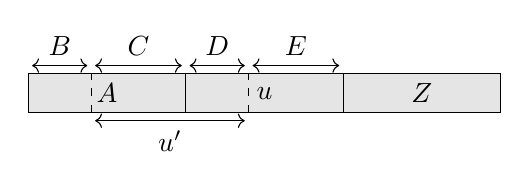
\begin{tikzpicture}
		\filldraw[fill=gray!20] (0,0) rectangle (2,0.5) node[midway] {$A$};
		\draw[<->] (0.05,0.6) -- (0.75,0.6) node[above,midway] {$B$};
		\draw[dashed] (0.8,0) -- (0.8,0.5);
		\draw[<->] (0.85,0.6) -- (1.95,0.6) node[above,midway] {$C$};
		\draw[solid] (2,0) -- (2,0.5);
		\filldraw[fill=gray!20] (2,0) rectangle (4,0.5) node[midway] {$u$};
		\draw[<->] (2.05,0.6) -- (2.75,0.6) node[above,midway] {$D$};
		\draw[<->] (0.85,-0.1) -- (2.75,-0.1) node [below,midway] {$u'$};
		\draw[dashed] (2.8,0) -- (2.8,0.5);
		\draw[<->] (2.85,0.6) -- (3.95,0.6) node[above,midway] {$E$};
		\filldraw[fill=gray!20] (4,0) rectangle (6,0.5) node[midway] {$Z$};
	\end{tikzpicture}\par}

	Then we have rules $CD \to v'$ and $DE \to v$ in $R$, so by hypothesis there is a $z \in A^*$ such that $v'E \to^*_R z$ and $Cv \to^*_R z$, and we have a common descendant like so: \[
		\begin{array}{lllll}
			& & Bv'EZ & & \\
			& \nearrow & & \searrowstar & \\
			a = BCDEZ & & & & BzZ. \\
			& \searrow & & \nearrowstar & \\
			& & BCvZ & &
		\end{array}
	\]

	\textbf{Case (iii)}: $u'$ is entirely contained in $u$. Factor $a = ABu'CZ$ so that $u = Bu'C$. Then by hypothesis there is a $z \in A^*$ such that $v \to^* z$ and $Bv'C \to^* z$. So we have the diagram: \[
		\begin{array}{lllll}
			& & ABv'CZ & & \\
			& \nearrow & & \searrowstar & \\
			a = ABu'CZ & & & & AzZ. \\
			& \searrow & & \nearrowstar & \\
			& & AvZ & &
		\end{array}
	\]

	\textbf{Case (iv)}: $u'$ is contained in $uZ$ but not in $u$ or $Z$. Factor $a = ABCDE$ as below, so that $u = BC$, $u' = CD$ and $Z = DE$:

	{\centering
	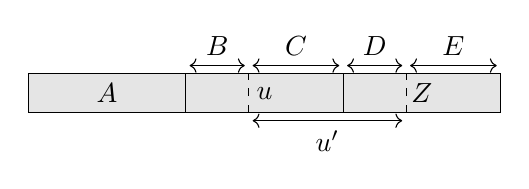
\begin{tikzpicture}
		\filldraw[fill=gray!20] (0,0) rectangle (2,0.5) node[midway] {$A$};
		\draw[<->] (2.05,0.6) -- (2.75,0.6) node[above,midway] {$B$};
		\draw[<->] (2.85,0.6) -- (3.95,0.6) node[above,midway] {$C$};
		\draw[solid] (2,0) -- (2,0.5);
		\filldraw[fill=gray!20] (2,0) rectangle (4,0.5) node[midway] {$u$};
		\draw[<->] (4.05,0.6) -- (4.75,0.6) node[above,midway] {$D$};
		\draw[dashed] (2.8,0) -- (2.8,0.5);
		\draw[<->] (4.85,0.6) -- (5.95,0.6) node[above,midway] {$E$};
		\filldraw[fill=gray!20] (4,0) rectangle (6,0.5) node[midway] {$Z$};
		\draw[dashed] (4.8,0) -- (4.8,0.5);
		\draw[<->] (2.85,-0.1) -- (4.75,-0.1) node [below,midway] {$u'$};
	\end{tikzpicture}\par}

	Since we have rules $BC \to v$, $CD \to v'$, by hypothesis there is a $z \in A^*$ such that $vD \to^* z$ and $Bv' \to z$, giving the diagram: \[
		\begin{array}{lllll}
			& & AvDE & & \\
			& \nearrow & & \searrowstar & \\
			a = ABCDE & & & & AzZ. \\
			& \searrow & & \nearrowstar & \\
			& & ABv'E & &
		\end{array}
	\]

	\textbf{Case (v)}: $u'$ is entirely contained in $Z$. This case is very similar to case (i) and is omitted.
\end{proof}


\begin{itemize}
	\item[Proposition] In a confluent rewriting system a string has at most one irreducible descendant.
\end{itemize}

\subsection{Normal forms}

\begin{itemize}
	\item[Proposition] Confluent noetherian rewriting systems give unique normal forms.
	\item When is the normal form computable?
\end{itemize}

\section{The word problem for special monoids} \label{sec:special-monoids}

In this section, we discuss the word problem for a special class of one-relation semigroups, namely `special' one-relation monoids.

\begin{defn} \label{def:special}
	A monoid $M$ is \dn{special} if it has a presentation of the form $\langle A \mid w_1 = \epsilon, w_2 = \epsilon, \ldots, w_n = \epsilon \rangle$ for nonempty words $w_i \in A^*$.
\end{defn}

The main result is a theorem of Adjan, which states that the word problem is indeed decidable for one-relation special monoids:

\begin{theorem}[Adjan] \label{thm:ors-decidablewp}
	Let $M$ be a one-relation special monoid, i.e. a monoid admitting a presentation of the form $\langle A \mid w = \epsilon\rangle$, where $A$ is an alphabet, $w \in A^+$. Then $M$ has decidable word problem.
\end{theorem}

Here, we follow Zhang's proof from \cite{Zhang1992a}. Zhang's overall approach is to construct a one-relation presentation for the group of units of the special monoid --- whose word problem is then decidable by Magnus' theorem --- and reduce the word problem of the whole monoid to that of the group of units using a confluent, noetherian rewriting system.

In another paper (\cite{Zhang1992}), Zhang uses a similar method to generalise this statement by reducing the word problem of any special monoid to the word problem of its group of units, as well as obtaining similar results on the conjugacy and divisibility problems for these monoids.


\subsection{Constructing a generating set}

Suppose $M = \langle A \mid w = \epsilon\rangle$ is a finitely presented monoid.

Given a subset $X \subseteq A^*$ of words, define
	\begin{align*}
		L(X) &= \{ x \in A^+ \mid \exists\ w \in A^* \colon wx \in X \} \text{ and } \\
		R(X) &= \{ x \in A^+ \mid \exists\ w \in A^* \colon xw \in X \}
	\end{align*}
to be the set of left and right factors respectively of words in $X$, and let $W(X) = L(X) \cap R(X)$ be the set of words which are both left and right factors each of some word in $X$.

Taking $C_1 = \{w\}$, let
	\[ C_{i+1} = C_i \cup \{ xy \mid y \in W(C_i), yx \in C_i \} \cup \{ yz \mid y \in W(C_i), zy \in C_i \} \]
be those words obtained by moving right factors from $W(C_i)$ to the beginning of the words in $C_i$ in which they appear and left factors to the end of words.

\begin{lemma}
	For each index $i$, every word in $C_i$ has the same length as $w$.
\end{lemma}
\begin{proof}
	This can be shown by a straightforward induction on $i$. It is true in $C_1$, since $C_1 = \{w\}$. So suppose every word in $C_i$ has length $|w|$, and let $xy$ be a new word in $C_{i+1}$ for some $x, y \in A^+$ such that $x$ or $y$ is in $W(C_i)$. Then either $xy$ or $yx$ in $C_i$ and hence $|xy| = |yx| = |w|$ by the inductive hypothesis. Hence every word in $C_{i+1}$ has length $|w|$ and so every word in $C_i$ has length $|w|$, for any index $i$.
\end{proof}

It follows from the above that since $|C_i| \le |A|^{|w|}$ (which is finite since $M$ is finitely presented) and $C_{i+1} \supseteq C_i$ for all $i \ge 1$, there is a maximal set $C_k$. Define a new set $E(M)$ to be those words in $W(C_k)$ which have no proper right factors in $W(C_k)$.

This set $E(M)$ will effectively serve as the generating set in the presentation for the group of units of $M$ which we construct in the remainder of the proof.

\subsubsection{An alternative definition}

In \cite{Zhang1992}, an alternative, non-constructive definition of a generating set for the group of units is given, based on the idea of \emph{minimal factors} of $w$.

\begin{defn}
	A word $v \in A^+$ is \dn{minimal} if:
	\begin{enumerate}[(i)]
		\item it is invertible in $M$,
		\item $|v| \le |w|$ and
		\item none of its nonempty prefixes are invertible in $M$.
	\end{enumerate}
\end{defn}

...


\subsection{Defining the presentation}

Define a new alphabet $B$ disjoint with $A$ such that we have a bijection $\midtilde\phi \colon E(M) \to B$, and let $\phi \colon E(M)^* \to B^*$ be the unique homomorphic extension of $\midtilde\phi$ to $E(M)^*$. By the following result, $\phi(w)$ is well-defined:

\begin{prop} \label{lma:relator-factors-E(M)}
	The relator $w$ is a product of factors in $E(M)$.
\end{prop}
\begin{proof}
	\hspace{-0.25mm}We show by induction on word length that every element of $W(C_k)$ is a product of factors in $E(M)$. First suppose that $u \in W(C_k)$ is of minimal length in $W(C_k)$. Then $u$ has no proper factors in $W(C_k)$, and so $u \in E(M)$.

	Now suppose that all strings in $W(C_k)$ with length less than $n$ are products of factors in $E(M)$, and let $u \in W(C_k)$ have length $n$. If $u$ has no proper right factors in $W(C_k)$, then it is in $E(M)$ by definition. Otherwise, we can write $u = ve$ for $e \in E(M)$, $v \in A^+$.

	We want to show that $v \in W(C_k)$, so that by the inductive hypothesis (since $|v| < n$), $v \in E(M)^*$ and hence $u \in E(M)^*$. Since $v$ is a prefix of $u$, for $v$ to be in $W(C_k)$ it remains only to show that it is a suffix of some word in $C_k$. Because $u \in W(C_k)$, there is some word $x \in C_k$ such that $x = x'u = x've$ . Then by the definition of $C_{k+1}$, since $e \in W(C_k)$, the word $ex'v \in C_{k+1}$. But $C_{k+1} = C_k$, so $v$ is indeed a suffix of a word in $C_k$.

	Altogether, this means $u$ is a product of factors in $E(M)$ and so by induction all the words of $W(C_k)$ are such a product. In particular, since $w \in W(C_k)$, $w$ is a product of factors in $E(M)$.
\end{proof}

We now define a monoid $M'$ given by the presentation $\langle B \mid \phi(w) = \epsilon \rangle$. We assert that this monoid is in fact a group:

\begin{prop}
	The monoid $M' = \langle B \mid \phi(w) = \epsilon\rangle$ is a group.
\end{prop}
\begin{proof}
	It suffices to show that every generator of $M'$ is invertible. We first show by induction that for all $i$, every word in $C_i$ is trivial in $M$. In the base case $C_1$, the only word to consider is $w$ itself, which is trivial by the defining relation $w = \epsilon$. Suppose then that all words in $C_j$ are trivial, for each $j \le i$, and consider a word $v \in C_{i+1}$, $v \not\in C_i$.

	This new word $v$ can arise in two ways. In the first case, $v = xy$ for some $y \in W(C_i)$, $yx \in C_i$. So by the inductive hypothesis, $yx =_M \epsilon$, i.e. $x$ is a right inverse for $y$ in $M$. As $y \in W(C_i)$, there is a word $u \in C_i$ such that $u = u'y =_M \epsilon$ for some $u' \in A^*$. So $u'$ is a left inverse for $y$ in $M$. We have a left and a right inverse for $y$ in $M$, so they must be equivalent in $M$, hence $v = xy =_M u'y =_M u$. But $u$ is in $C_i$ and so is trivial by the inductive hypothesis. Therefore $v =_M \epsilon$ as required.

	A similar argument shows that $v$ is trivial in $M$ if $v = yz$ for $y \in W(C_i)$, $zy \in C_i$. This accounts for every word in $C_{i+1}$, and so by induction all words in $C_j$ are trivial in $M$, for every index $j$. In particular, all the words in $C_k$ are trivial.

	For any word $z \in W(C_k)$, there are words $a, b$ in $C_k$ such that $a = za'$ and $b = b'z$ for some $a', b' \in A^*$. Since these words $a$ and $b$ are trivial in $M$, $a'$ is a right inverse for $z$ and $b'$ is a left inverse for $z$ in $M$ and hence $z$ is invertible in $M$. In particular, it follows that every word in $E(M)$ is invertible.

	To conclude, let $b \in B$ be a generator of $M'$. Then $\tilde\phi^{-1}(b) \in E(M)$ has an inverse $\midbar b$ in $M$. Hence $\epsilon =_M \tilde\phi^{-1}(b) \midbar{b}$ and so $\epsilon =_{M'} b\phi(\midbar{b})$; and likewise $\phi(\midbar{b})b = \epsilon$. The arbitrary generator $b$ of $M'$ is hence invertible, so $M'$ is a group.
\end{proof}

We assert further that it is, as suggested, the group of units of $M$.

\begin{theorem}
	The monoid $M'$ is isomorphic to the group of units of $M$.
\end{theorem}

In light of this, we shall henceforth refer to the monoid $M'$ as $G$.

\subsection{The rewriting system}

Let $\prec$ be some linear order on the alphabet $A$, and extend it to a shortlex order $<$ on $A^*$. Then define a rewriting system $R$ on $A^*$ by
	\[ R = \{ (u, v) \mid u, v \in E(M)^*, v < u, \phi(u) =_G \phi(v) \}. \]

We note immediately that $R$ is noetherian: since if $(u, v)$ is a rule in $R$, then we must have $v < u$, and the short-lex order $<$ is a well-founded relation by a result from the previous section.

This system $R$ is equivalent to the system $\{(w, \epsilon)\}$, i.e. they present the same monoid:
\begin{lemma} \label{lma:R-equivalent-to-pres}
	The rewriting systems $\{(w, \epsilon)\}$ and $R$ are equivalent in the sense that their induced congruences  are equal, and hence that $\langle A \mid w \rangle$ = $\langle A \mid \{u = v : (u, v) \in R\}\rangle$.
\end{lemma}
\begin{proof}
	First, observe that $w \in E(M)^*$ by \cref{lma:relator-factors-E(M)}; $\epsilon < w$; and $\phi(w) =_G \epsilon$ follows immediately from the presentation for $G$, so $(w, \epsilon)$ is a rule in $R$ and hence $\leftrightarrow^*_{\{(w,\epsilon)\}}\ \subseteq\ \leftrightarrow^*_R$.

Conversely, suppose $(u, v)$ is a rule in $R$. Then $\phi(u) =_G \phi(v)$ means $\phi(u) \leftrightarrow^*_{\{(\phi(w), \epsilon)\}} \phi(v)$, and since $\phi$ is a homomorphism, $u \leftrightarrow^*_{\{(w, \epsilon)\}} v$. So $\leftrightarrow^*_R\ \subseteq\ \leftrightarrow^*_{\{(w,\epsilon)\}}$.

Hence the two rewriting systems are equivalent.
\end{proof}


\subsubsection{\texorpdfstring{Some lemmas on $E(M)$}{Some lemmas on E(M)}}

We state here two lemmas about the generating set $E(M)$ which will be useful to prove that $R$ is confluent:

\begin{lemma} \label{lma:no-middle-E(M)}
	If $x, y, z \in A^*$ are strings such that $xy, yz \in E(M)$, then either $y = \epsilon$ or $x = z = \epsilon$.
\end{lemma}
\begin{proof}
	Suppose $y \ne \epsilon$. Then since $xy \in E(M)$, $xy \in W(C_k)$ and in particular, $xy \in L(C_k)$, so there is some $\alpha \in A^*$ such that $\alpha x \cdot y \in C_k$. So $y$ is a right factor of a word in $C_k$, i.e. $y \in R(C_k)$. Likewise, $yz \in R(C_k)$ so $y \cdot z\beta \in C_k$ for some $\beta \in A^*$ and $y \in L(C_k)$. Hence $y \in W(C_k)$. By the definition of $E(M)$, $xy$ has no proper right factor in $W(C_k)$, so $y$ must not be a proper factor; but by assumption, $y \ne \epsilon$, so we must have $x = \epsilon$. Similarly, $yz$ has no proper right factor in $W(C_k)$, so $z$ is not a proper factor and $z = \epsilon$.
\end{proof}

\begin{cly} \label{cly:middle-E(M)*}
	If $x, y, z \in A^*$ are strings such that $xy, yz \in E(M)^*$, then $y \in E(M)^*$.
\end{cly}


\subsubsection{\texorpdfstring{Confluence of $R$}{Confluence of R}}

We apply \cref{thm:confluent-cond} directly to $R$ to show that it is locally confluent. Since $R$ is noetherian, by \cref{thm:newman} this suffices to show $R$ is confluent.

For part \ref{it:conf-overlap}, suppose $uv \to_R x$ and $vw \to_R y$, with $uv \ne vw$ (if they are equal, we have nothing to prove). We claim that in fact one of $xw \to uy$ or $uy \to xw$ is a rule in $R$ and so $uy$ or $xw$ is a suitable $z$. By the definition of $R$, $uv, vw, x, y\in E(M)^*$, and so by \cref{cly:middle-E(M)*}, $v \in E(M)^*$. Hence $u, w \in E(M)^*$ and $uy, xw \in E(M)^*$. Now observe that by the rules we know are in $R$ and the fact $\phi$ is a homomorphism, we have $\phi(xw) = \phi(x)\phi(w) =_G \phi(uv)\phi(w) = \phi(u)\phi(vw) =_G \phi(u)\phi(y) = \phi(uy)$. Finally, since $<$ is linear, either $xw < uy$, in which case $uy \to xw$ is a rule in $R$; or $uy < xw$, in which case $xw \to uy$ is a rule in $R$ as required.

Now consider condition \ref{it:conf-middle}: suppose $uvw \to_R x$ and $v \to_R y$, and again assume that $v \ne y$. Observe that $\phi(x) =_G \phi(uyw)$, since $\phi(uvw) =_G \phi(x)$ and $\phi(v) =_G \phi(y)$. Furthermore, either $uyw < x$ or $x < uyw$. So as before, if $uyw \in E(M)^*$, then one of $x$ or $uyw$ will be a suitable $z$. Since $uvw, v, y \in E(M)^*$, if $uyw \not\in E(M)^*$, then $u = u_1u_2 \cdots u_m U$ and $w = W w_1 w_2 \cdots w_n$ for $u_i, w_i \in E(M)$ and some non-empty strings $U$ and $W$, with $UvW \in E(M)$. This means $v$ must be shorter than the longest word in $E(M)$ (or $UvW$ would be longer and therefore not in $E(M)$).

The following lemma completes the proof:

\begin{lemma} \label{lma:shorter-irreducible}
	Any word $a \in A^*$ shorter than the longest word in $E(M)$ is irreducible by $R$.
\end{lemma}
\begin{proof}
	Let $L$ be a word of maximal length in $E(M)$, and suppose $a$ were reducible. Then we can write $a = a'ba''$ where $b \in E(M)^*$ and $b \to_R c$ for some $c \in E(M)^*$. Then $c < b$ and so $|c| \le |b| \le |a| < |L|$, and hence $L$ cannot appear in $b$ or $c$.
	
	We then recall the Freiheitssatz for one-relator groups (\cref{thm:freiheitssatz}).	Since $b \to_R c$, $\phi(b) =_G \phi(c)$. Then as $L$ is not in $b$ or $c$, $\phi(L)$ is not in $\phi(b)$ or $\phi(c)$, i.e. $\phi(b)$ and $\phi(c)$ are in the subgroup of $G$ generated by $B \setminus \{\phi(L)\}$. This is free by the Freiheitssatz, and so $\phi(b) = \phi(c)$ as words. Since $\phi$ is a homomorphism and $\midtilde\phi$ is a bijection, $\phi$ is injective and so $b = c$. But $c < b$, so we have a contradiction and $a$ is indeed irreducible.
\end{proof}

It follows from this that $v$ is irreducible by $R$; but this is impossible, since by hypothesis $v \to_R y$. So in fact $uyw \in E(M)^*$, and one of $uyw \to_R x$ or $x \to_R uyw$ holds. Therefore condition \ref{it:conf-middle} is satisfied and $R$ is confluent.


\subsection{The word problem is decidable}

We can now prove \cref{thm:ors-decidablewp}. Suppose we have two words $u$ and $v \in A^*$. Observe that we can enumerate the rules of $R$ which could apply to $u$ in a finite number of steps: since if a rule $(a, b)$ applies to $u$, then $a$ is a substring of $u$ and so $|b| \le |a| \le |u|$. Enumerating all possible pairs $(a, b)$ of strings in of length $|u|$ or less, it is decidable whether $b < a$ and --- by \cref{thm:orgp-decidablewp} --- whether $a =_G b$, and hence whether $(a, b)$ is a rule in $R$. If there are any such rules, we can apply one and repeat the process with the resulting string. Eventually, since $R$ is confluent and noetherian, no such rules shall remain and we will have computed the unique normal form $\midbar{u}$ for $u$.

Repeating this process starting with $v$, we can compute its normal form $\midbar{v}$ in a finite number of steps. Since $R$ is equivalent to $\{(w, \epsilon)\}$ by \cref{lma:R-equivalent-to-pres}, $u =_M v$ if and only if $\midbar{u} = \midbar{v}$ as words. We can perform this comparison in a finite number of steps, so the overall problem of determining whether $u =_M v$ is decidable. This is precisely the word problem for $M$.


\printbibliography

\printindex

\end{document}
